\documentclass[8pt]{beamer}
    \usepackage{graphicx}
    \usepackage{wrapfig}
    \usepackage{multicol}

    \usepackage[T1]{fontenc}
    \usepackage{mathptmx}
    \usetheme{Madrid}
    
    \title{Dog training - Independent}
    \author{Ahmed Ayman}
    
    \begin{document}
        \maketitle
        \begin{frame}{Agenda}
            \begin{itemize}
                \item Problem definition
                \item Questions and the test
                \item Assumption checks
                \item Results and final thoughts
            \end{itemize}
        \end{frame}

        \begin{frame}{Problem definition}
            \textbf{There are two popular methods to train dogs}
            \begin{itemize}
                \item clicker: Make sound when the dog do something right
                \item food: The dog get some food after doing something right
            \end{itemize}
            \textbf{a dog trainer would like which one is better}\\
            \textcolor{red}{We hope there is a difference between the two methods \textbf{(Statistically significant)}}\\[.5cm]
            \begin{figure}
                \centering
                
\includegraphics[width=.2\textwidth]{images/clicker.jpg}
                \vspace{.25cm}
            \end{figure}

            \begin{figure}
                \centering
                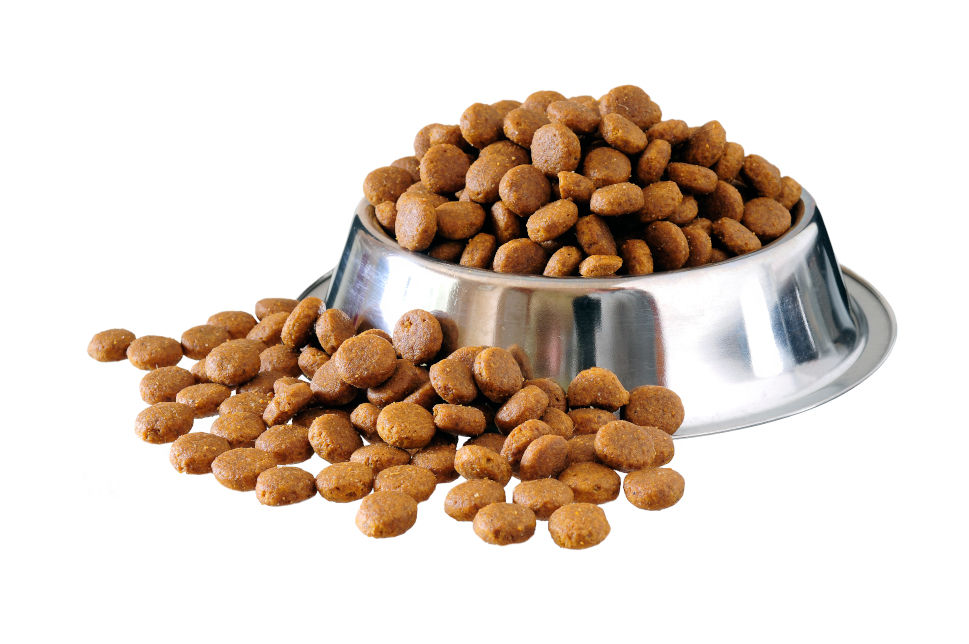
\includegraphics[width=.2\textwidth]{images/dry_food.jpg}
            \end{figure}
        \end{frame}

        \begin{frame}{Questions and the test}
            \begin{block}{\textbf{Questions}}
                \begin{itemize}
                    \item \textbf{Business:} Are the two training methods have the same effectiveness
                    \item \textbf{Statistical:} Score(dog with clicker-training) = Score(dog with food-training)
                \end{itemize}
            \end{block}

            \begin{block}{\textbf{The test}}
                The Statistical test is \textcolor{red}{\textbf{Independent t-test}}\\
                This test requires some assumptions check \\ 
                \begin{itemize}
                    \item Are the two groups have similar variance 
                    \item Is the data Normally distributed
                    \item \textcolor{red}{We hope those tests to be \textbf{(Statistically not significant)}}
                    \item To be able to do the t-test
                \end{itemize}
            \end{block}
        \end{frame}

        \begin{frame}{Assumption checks}
            \begin{columns}
                \column{.45\textwidth}
                \begin{itemize}
                    \item The p-value of \textbf{Shpiro-test} < .05
                    \item which means: The data Normally distributed: \textcolor{blue}{\textbf{Great}}
                    \item The p-value of \textbf{Levene-test} < .05
                    \item which means: The groups have similar variance: \textcolor{blue}{\textbf{Great}}
                \end{itemize}
                \column{.55\textwidth}
                \begin{figure}
                    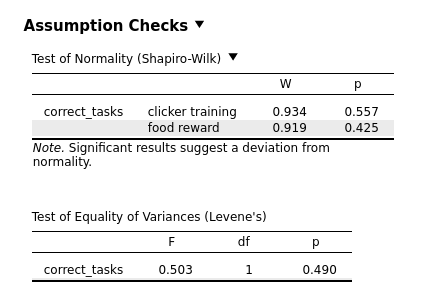
\includegraphics[width=.95\textwidth]{images/indep assumptions.png}
                    \vspace{.25cm}
                \end{figure}
            \end{columns}
        \end{frame}

        \begin{frame}{Results and final thoughts}
            \begin{columns}
                \column{.45\textwidth}
                \begin{itemize}
                    \item Although there is a difference we can see with our eyes
                    \item And the \textbf{Effect size} is large
                    \item But, we can't reject the $H_0$
                    \item As \textbf{p-value > .05}
                    \item \textcolor{red}{\textbf{Sad}}
                \end{itemize}
                \column{.55\textwidth}
                \begin{figure}
                    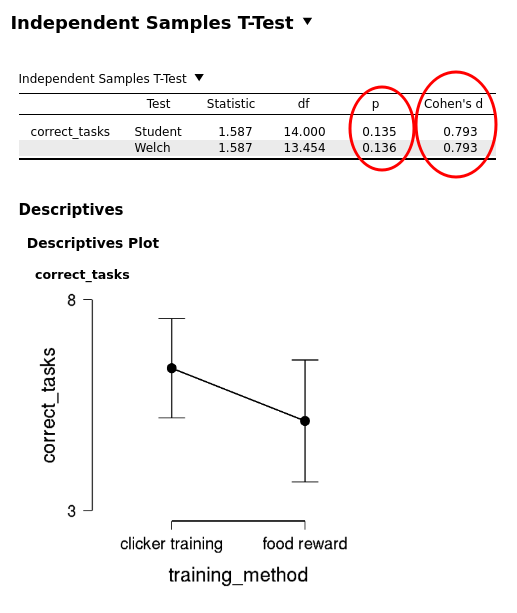
\includegraphics[width=.95\textwidth]{images/indep result.png}
                    \vspace{.25cm}
                \end{figure}
            \end{columns}
        \end{frame}
    \end{document}